%Zero.tex
\chapter{Zero}\label{char:Zero}
Zero is the deuteragonist of the X series. A close friend of X, Zero acts as a counterpart for him, opposing X's kindness and uncertainty with a cold and emotionless attitude, often taking action without hesitating. However, behind his attitude Zero hides a kind but wounded soul~\cite{wiki:Zero} which cares for his friends.

\begin{figure}[htp]
	\centering
	
\includegraphics[height=\BIGportraitsize]{figures/Characters/Char_Z_2.png}	
	
\includegraphics[height=\portraitsize]{figures/Characters/Char_Z.png}
	\caption{Zero (first and after X2).}
\end{figure}

\section{Creation}
Just as X is the last and best creation of Dr.~Light, Zero is the last creation of Dr.~Wily, fulfilling the doctor's dream of creating the strongest robot ever. 
Just like for X, precise information about Zero's creation or specifications are not given. The first instance of Wily talking about Zero's project can be found in Bass' ending in \textit{Mega Man: The Power Battle}, where Wily discusses with Bass about his new project, a robot capable of easily disposing of Bass himself as well as the original Mega Man\footnote{\textit{The robot I'm making right now will blow the both of you away}- Dr.~Wily, Bass ending, Mega Man: The Power Battle}. Then, in the following entry in the series, \textit{ Mega Man 2: The Power Fighters}, this discussion is resumed again, with Wily talking about how he managed to learn from his mistakes, which led him to developing a new type of robot, by combining together the accidental discovery of the bassium energy as a power source or the study of both Proto Man~\cite{art:mmnetwork:24_mavs} and Mega Man:
\begin{quote}
	``I studied Megaman hoping to create a similar robot. Then I developed a powerful energy called "Bassnium" purely by accident. Thus, I created you Bass. Currently Bassnium is the most powerful energy on Earth. But, that's not for long. Hee hee, I've learned from my accident... And I've created a new type of robot which is much more powerful than you or Megaman! It'll be some time before I complete this project though. You better get ready!"'' - Dr. Wily, Bass ending, Mega Man 2: The Power Fighters
\end{quote}
On such occasion, Wily also shows the blueprint of his project, a shadowy silhouette of Zero with his appearance from X2 onward.

\begin{figure}[htp]
	\centering
	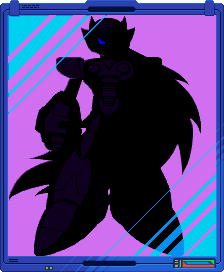
\includegraphics[height=4cm]{figures/Characters/MM2TPF_Zero.png}
	\caption{Zero's schematics during the Bass ending in Mega Man 2: The Power Fighters}
\end{figure}

Wily’s plans, however, do not work as intended, as Zero turns out to suffer from a critical flaw in his cognitive program that makes him uncontrollably violent and unwilling to obey orders. As a result, Wily is forced to seal Zero inside a capsule together with a special virus program, the \emph{Robot Destroy Program}\footnote{Official name given in Mega Man X Dive - 2020} which, although never explicitly stated, is supposed to be originally meant to act as a corrective patch for Zero’s brain, designed to infect him upon awakening and stabilize his systems, to unlock his full potential.
\begin{figure}[htp]
	\centering
	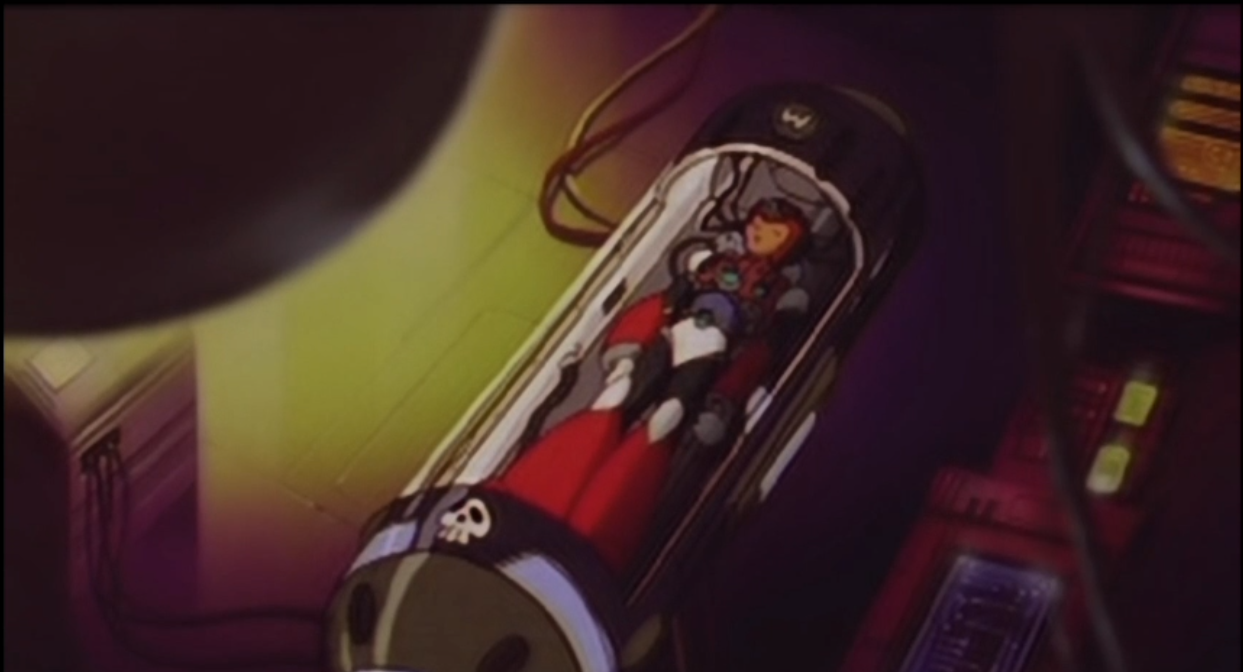
\includegraphics[height=4cm]{figures/X4/Story_Z_00.png}
	\caption{Flashback of Zero's construction}
\end{figure}
According to early drafts of the X saga’s storyline~\cite{art:mmnetwork:24_mavs}, Dr.~Wily does not live long enough to complete his project, leaving both Zero and the program sealed away for a hundred years, while also finding a way to let his consciousness live on~\cite{blog:Inafune}. While this has never been officially confirmed or denied, the fact that Zero appears in an incomplete state up to the second game, where is repaired and upgraded by Serges (chapter~\ref{char:Serges}) seems to indirectly supports this theory.


Although Zero remains dormant within the capsule for decades, the program stored alongside him begins leaking into the environment, slowly spreading across the world. Being a virus, it starts infecting other machines, Reploids included, altering their systems and causing behaviors comparable to Maverick tendencies. It is possible to speculate that this corruption arises from the combination of the virus’s inherent purpose—to rewrite machine logic—and the imperfect emotional circuit Dr.~Cain failed to replicate from X’s design, which provides an ideal vulnerability for infection. Due to its devastating effects, the Robot Destroy Program becomes known as the \emph{Maverick Virus}, the original strain of what would later evolve into the Sigma Virus.

Roughly a century after being sealed, Zero’s capsule is discovered by a group of Reploids investigating the abandoned laboratory. Unwillingly, they reactivate the still flawed Zero, who immediately attacks and annihilates the entire team along with anyone else who dares to enter his lair. Deemed a major threat to humans, Zero is quickly classified as a Maverick—the infamous ``Red Maverick''. The Gamma Unit of the Maverick Hunters is therefore dispatched to neutralize him, but the attempt ends in failure as Zero effortlessly destroys the entire squad. As such, to prevent further casualties Maverick Hunter Commander Sigma decides to face the mysterious Maverick himself, engaging Zero in a one-on-one battle. Despite Sigma’s formidable strength, however, Zero manages to overpower him, severely injuring and toy with him while laughing maniacally. However, because their duel takes place inside the abandoned lab, both of them are exposed to massive amounts of the Maverick Virus leaking from the capsule which, detecting its intended host, begins reprogramming Zero’s systems causing intense pain and making a pulsating ``W'' symbol appear within the gem on his forehead. Taking advantage of this moment of weakness, Sigma lands a decisive blow, shattering the gem and knocking Zero down. Following the encounter, Sigma delivers the unconscious Zero to Dr.~Cain for study, though what happens immediately afterward remains unknown.

While not confirmed,it is possible to speculate that, upon awakening, Zero emerges as a completely different individual, now with his serious and composed attitude characterizing him throughout the X saga. Ultimately  Zero joins the Maverick Hunters under Sigma’s command.

Although no official explanation is ever given, it is widely speculated that Zero's change of personality can tracked down to Sigma’s strike interrupting the reprogramming process midway, resulting in the virus successfully stabilized Zero’s violent tendencies but failing to fully awaken his original personality. This fact could also be the cause of Zero suffering occasionally for vision similar to nightmares, were he would see the shadows of his creator ordering him to fulfill his duty and destroy ``his enemy''.
\begin{figure}[htp]
	\centering
	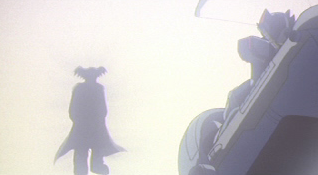
\includegraphics[height=4cm]{figures/X4/story_Z_1.png}
	\caption{Zero's vision of his creator}
\end{figure}
Nonetheless, Zero remains infected with the Robot Destroy Program, unintentionally serving as a vector for the disease and enabling its continued spread throughout the world as he fulfills his duties as a Hunter~\cite{book:RMZ_Complete_works}.


\section{The X saga and the Maverick Wars}
As Sigma go Maverick, Zero is appointed as leader of the Maverick Hunters, being the highest in rank remained within the group. He then proceeds to lead the organization against Sigma, entrusting X to deal with Sigma's subordinates while he tries to locate the enemy fortress. The two manage to complete their task simultaneously, and reunite to attack Sigma together, Zero acting as decoy due him being more powerful than X, to let him sneak inside unnoticed. Once in they briefly reunite but are interrupted by Vile which Zero  challenges to a duel, only to be caught in a trap Vile had previously prepared. Vile then proceeds to use him as a hostage and manages to capture X too, but Zero breaks free and, in order to save his friend, explodes to take down Vile too, but only manages to destroy his Ride armor. His action, however, gives X the strength necessary to break free and take Vile down definitively. With his last words Zero encourages X to proceed and face Sigma, firmly believing he has the power to beat him.

Although destroyed, Zero's control circuit remains miraculously intact and is stored at the Maverick Hunters Headquarter. Zero's body (or what remains of it) is instead recovered by the X-Hunters, which tasks Serges to repair it. Serges not only repairs Zero's body, but also upgrades it into its final version, adding the missing shoulder pads and giving him his iconic Z-Saber. For the whole duration of the X-Hunters operation Zero remains incomplete, as the two key components stay in the hands of the two opposing factions. It is only near the end that Zero is resurrected, depending on the action X takes while fighting the X-Hunters. Zero can either be saved by X, who had previously won Zero's body parts from the X-Hunters, and be repaired by Dr.~Cain, or can be resurrected by Serges, after the X-Hunters steal the control circuit from the Maverick Hunters HQ. In the former case he reunites with X shortly before the final fight, just in time to destroy his clone, while in the latter case he will be put under Sigma's control and will fight X, which has to defeat him and make him come to his senses. Whichever the case is, Zero aids X during the final confrontation with Sigma, by destroying the main computer Sigma is using to spread his virus around the world. Following his resurrection, Zero is reintegrated within the hunters ranks, although as leader of the 0th division, since X was promoted leader of the 17th in his place. 

During the event also known as the ``Doppler Incident'', Zero is sent alongside X to dispose of Doppler's mavericks and secure the evil scientist to justice. However, they are initially forced to retreat, as Doppler's forces were attacking directly the maverick hunter's headquarter. In such occasion X is capture by former hunter Mac, but Zero manages to save him and kills the former hunter. After saving their base, X and Zero return to their mission in Doppler Town. There they manage to defeat all Doppler's mavericks, including the nightmare police and a revived Vile. Ultimately, after even Doppler has been taken down by X, the two split: X must face Sigma, the true mastermind behind all the situation, while Zero focuses on destroying the laboratory power generator. In one of the possible endings. Zero also manages to rescue X from being possessed by Sigma, first imbuing his sword with Doppler's antivirus and later by striking Sigma in his back, causing him to disappear.

A major turn point for Zero's character happens during the time period later known as the ``Great Repliforce War'' in which Zero takes a decisive part. The start of Zero's tragedy begins when mavericks seemingly belonging to Repliforce started attacking the flying city of Sky Lagoon, where Zero is sent to end the fights. However, Zero arrives too late, finding out the city's main generator is irreparably damaged and the city is doomed to fall, therefore forcing him to quickly escape to not get caught in the crash. Following such incident, Zero continues investigating the wreckage, where he find an injured Iris under attack from a massive mechaniloid, which Zero quickly dispose of. Upon saving her, Zero is reached by Colonel, Iris' brother who was searching for her and who thanks Zero for having saved his sister. Zero, however, questions Colonel on Repliforce activity in the area, and asks him to disarm and follow for interrogation on the facts. Colonel, being a pride soldier, refuse to obey, thus forcing high ranks of society to label all Repliforce as mavericks, to which they reply by declaring independence and starting preparation to create a reploid-only nation in space. As such, the clash between Repliforce and the Hunters becomes inevitable, Zero being in the front line dealing with repliforce high commanders. Alongside him remains Iris, who refuse any form of violence, helping Zero for as much as she can to limit casualties across the two parts, fearing to loose his beloved brother or Zero in the fight. Zero, on the other hand, fights merciless, being moved by a deep hatred for mavericks.

The first fracture between Iris and Zero appears when Colonel challenges Zero to a duel, determined to avenge his fallen comrades and dispose of a potential threat to their plans. When the two meet, Iris intervenes, reminding Colonel that Zero once saved her life and asking him to honor his debt. As such, Colonel retreats, leaving Iris who keeps trying to dissuade Zero from fighting her brother, but without success, as the hunter remains resolute in his mission.  
Not so long after, in fact, the two warriors cross paths again at the spaceport, where Colonel stayed behind to protect Repliforce’s retreat to the orbital station known as \emph{Final Weapon}. This time, Iris does not intervene in time, and the confrontation turns into a mortal duel where Zero ultimately prevails, fatally wounding Colonel who, with his dying breath, asks Zero to deliver a final message to Iris, assuring her that he died peacefully as a true soldier. However, Zero never gets the chance to fulfill this request, as upon returning to headquarters he learns that Iris has departed for space with Repliforce.  

Determined to find her, Zero rushes to Final Weapon, only to be confronted by Iris herself, consumed by grief over her brother’s death and now siding fully with Repliforce, resolute to stop him. To do so, she installs Colonel’s core chip within her body, transforming into the ``Ultimate Battle Reploid'' (see~\ref{char:Iris}) but is ultimately overwhelmed by the power flowing through her,  losing control and forcing Zero to fight her. After a fierce struggle, Zero defeats Iris and restores her original form, but at the cost of her life. Holding the dying Iris in his arms, Zero listens as she confesses her true wish: to live peacefully in a world inhabited only by Reploids, together with her brother and Zero. Overcome by grief, Zero screams in despair, questioning the purpose behind all his battles.  
\begin{figure}[htp]
	\centering
	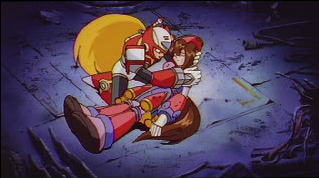
\includegraphics[height=4cm]{figures/X4/story_Z_5.png}
	\caption{Zero holding Iris}
\end{figure}

Still burdened by sorrow, Zero advances deeper into the fortress to confront General, whom he blames for Iris’s fate. As the two meet, they immediately engage in battle, each guided by their convictions, until Zero corners and gravely injures the Repliforce leader. Before Zero can strike the final blow, however, the space station begins operating autonomously and without General's order, its cannon starting to lock onto Earth. Recognizing the danger, General asks Zero to continue forward and reach the station's  core to stop the weapon. Once there, he discovers that Sigma is once again behind the chaos, the Maverick revealing himself as the true mastermind of the war, and therefore responsible for the deaths of both Colonel and Iris, and taunting Zero by saying that killing is his true nature, reminding him of their first encounter when their roles were reversed and Zero was the Maverick. Despite Sigma’s words, Zero remains steadfast and defeats him, destroying his bodies once again.  However, Sigma manages to delay Zero long enough for the cannon to reach the point of no return, leaving no time to disable it. In a final act of redemption, General reappears, grievously wounded, and bids Zero farewell before throwing himself into the cannon’s beam, absorbing the blast and destroying Final Weapon in the process. As the fortress collapses, Zero escapes aboard a shuttle, his heart heavy with grief and doubt,  questioning what his true nature really is. 

